%%%
\documentclass[xcolor=dvipsnames, aspectratio=169]{beamer}
%\usepackage{beamerthemesplit, listings, verbatim}

%\usepackage[absolute,overlay,showboxes]{textpos}
\usepackage[absolute,overlay]{textpos}

\usepackage{fontspec}

\usepackage{graphicx,wrapfig}
\usepackage{amsfonts,amsmath, amssymb, latexsym, amsthm}
\usepackage{epsfig}
\usepackage{float,enumerate}
\usepackage{listings}
\usepackage{mathtools}
\usepackage{multicol}
\usepackage{pifont}
\usepackage{tikz}
\usepackage{tikz-3dplot}
\usetikzlibrary{arrows}
\usetikzlibrary{scopes}
\usepackage{ulem}
\usepackage{xcolor}


\definecolor{Blueprint}{RGB}{0,61,162}
\definecolor{DarkBlue}{rgb}{0.15,0.0,0.9}
\definecolor{Red}{rgb}{0.9,0.0,0.1}
\definecolor{Colortest}{rgb}{0.1,0.55,0.1}
\definecolor{Orange}{rgb}{0.75,0.3,0.3}
\definecolor{JBlue}{HTML}{08399F}
\definecolor{Purple}{HTML}{8243DB}
\definecolor{aocbg}{HTML}{0F1022}
\definecolor{aocfg0}{HTML}{1FCA23}
\definecolor{aocfg1}{HTML}{106319}

\setbeamertemplate{navigation symbols}{} % turns nav syms off
\setbeamercolor{background canvas}{bg=Blueprint}


%\title[Daily Notes]{A Beamer Template for notes}
%\subtitle[]{}
\author[JLP]{Jesse L. Patsolic}


\def\Title#1{\noindent{\large\textcolor{white}{\sf{#1}}}}
\def\MTitle#1{\noindent{\large\textcolor{white}{\tt{#1}}}}

\newcommand\Mygrid{%
\tikz[
  remember picture,
  overlay,
  color=white,
  yscale=-1,
  xstep=\TPHorizModule,ystep=\TPVertModule,
  yshift=\TPVertModule,xshift=0pt]
  \draw (current page.north west) grid (current page.south east);}

\begin{document}

%% Example of a full page figure.
\begin{frame}[plain]
%\Mygrid
%\begin{textblock}{11}(0,0)
%    \Title{Jesse Leigh Patsolic, B.S., M.A.}
%\end{textblock}
%\makebox[\linewidth]{\includegraphics[height=0.95\paperheight]{logoBig.png}}

%%% Middle Explainer Box
%\begin{textblock}{5}(5,4)
% \MTitle{%
% Consider the case where $\{A, A_1\}$ are synonyms and $\{A,B\}$ are a pair of keywords.
% }
%\end{textblock}

\begin{textblock}{5}(0,0)
  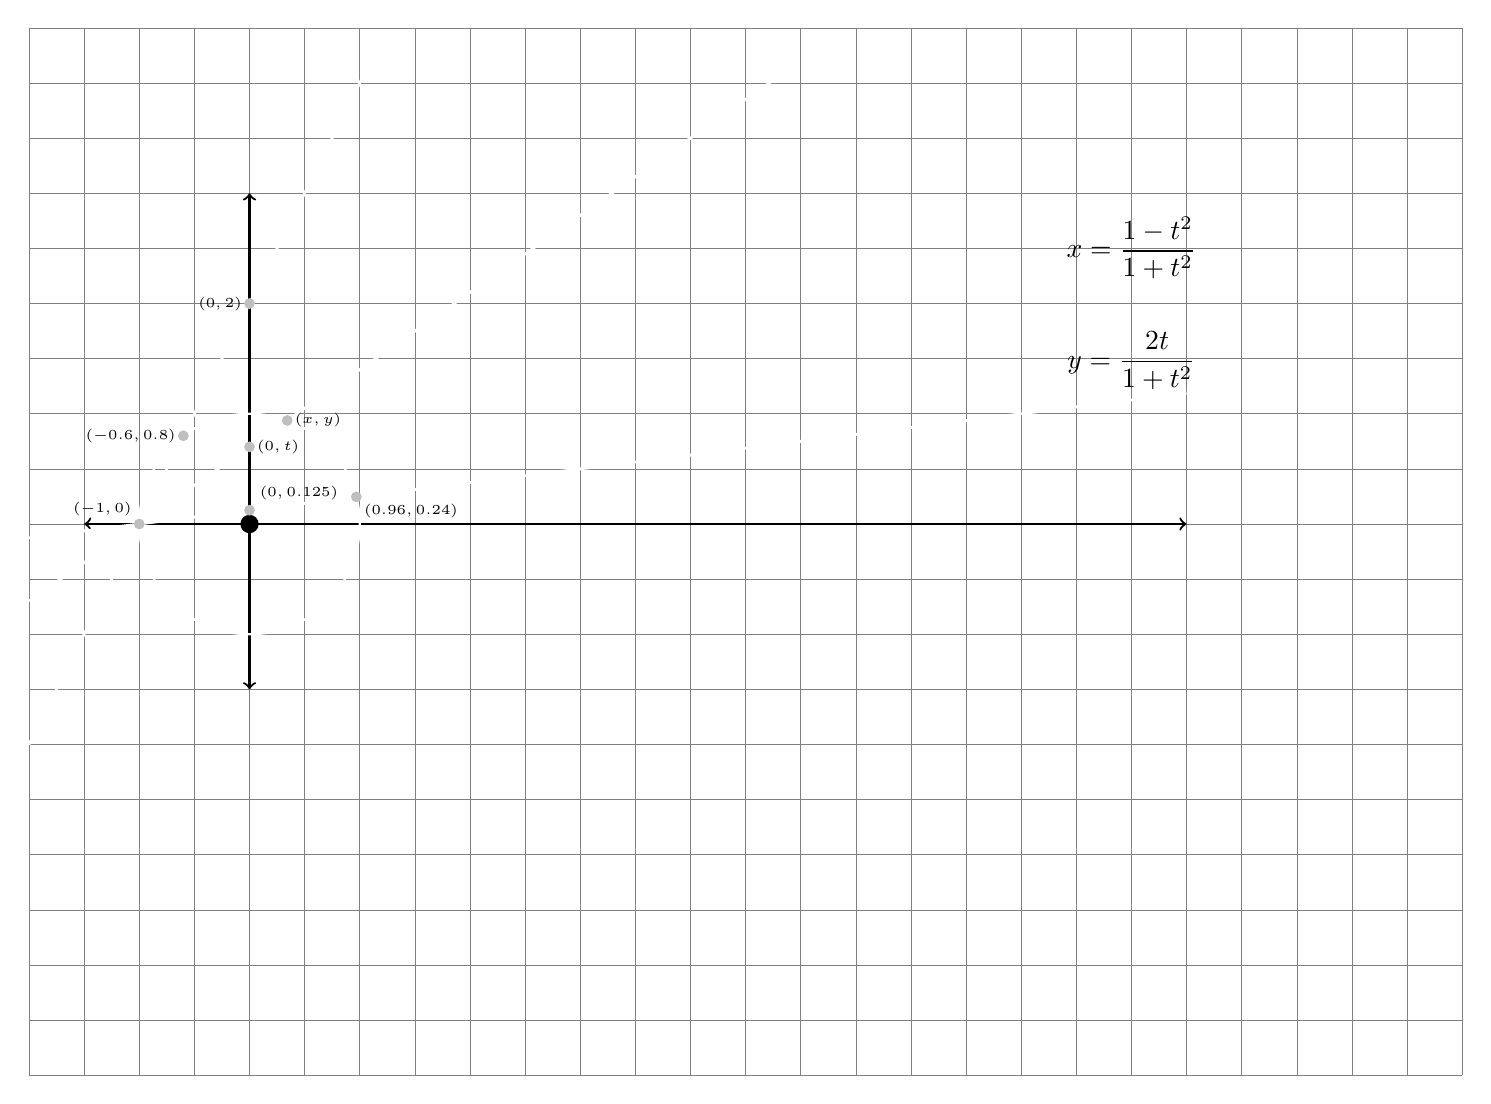
\begin{tikzpicture}[scale=1.4, color = white, line width=1]
      \draw[step=0.5cm, gray, very thin] (-5,5.5) grid (8,-4);
      \begin{scope}[xshift=-3cm,yshift=1cm]
        %axes
        \draw[thick, <->, color=black] (0,-1.5) -- (0,3);
        \draw[thick, <->, color=black] (-1.5,0) -- (8.5,0);

        \iffalse
        \foreach \x in {0,1,2,3,4,5,6,7} {
        \foreach \y in {1,2,3,4} {
          \draw[fill,color=black!20] (\x,\y) circle (2pt);
          \draw[node font=\tiny, anchor=west] (\x,\y) node {(\x, \y)};
          }
        }
        \fi

        \draw[fill,color=black] (0,0) circle (2pt);
        \draw[thick] (0,0) circle (1cm);
  
%        y = mx + b
%l1      
        \draw[smooth, samples=10, domain=-2:4.75] plot(\x, 0.7*\x + 0.7);
%l2
        \draw[smooth, samples=10, domain=-2:1.03125] plot(\x, 2*\x + 2);
%l3
        \draw[smooth, samples=10, domain=-2:8.5] plot(\x, 1/8*\x + 1/8);

        \draw[fill,color=gray!50] (-1,0) circle (1pt) node[above left,black, node font = \tiny] {$\left(-1,0\right)$};

        \draw[fill,color=gray!50] (0,0.7) circle (1pt) node[right,black, node font = \tiny] {$\left(0,t\right)$};

        \draw[fill,color=gray!50] (0.3423, 0.9396) circle (1pt) node[right,black, node font = \tiny] {$\left(x,y\right)$};

        
        \draw[fill,color=gray!50] (0,2) circle (1pt) node[left,black, node font = \tiny] {$\left(0,2\right)$};

        \draw[fill,color=gray!50] (-0.6,0.8) circle (1pt) node[left,black, node font = \tiny] {$\left(-0.6,0.8\right)$};

  
        \draw[fill,color=gray!50] (0,0.125) circle (1pt) node[above right=1pt,black, node font = \tiny] {$\left(0,0.125\right)$};
        \draw[fill,color=gray!50] (0.9692,0.2461) circle (1pt) node[below right,black, node font = \tiny] {$\left(0.96,0.24\right)$};

        \draw (8,2.125) node[above,black] {$x = \dfrac{1-t^2}{1+t^2}$};
        \draw (8,1.125) node[above,black] {$y = \dfrac{2t}{1+t^2}$};

        %\draw (8,-1) node[above,black] {Stereographic Projection of the circle with radius 1 to the real line (y-axis).};
      \end{scope}
  \end{tikzpicture}
\end{textblock}

\begin{textblock}{14}(0.25,2)
  \uline{Stereographic Projection of the circle with radius 1 to the real line (y-axis).}
\end{textblock}

\end{frame}

\end{document}
%%%
%%% TIME: 
%%% WORKING STATUS:
%%% COMMENTS:
